% !Mode:: "TeX:UTF-8"
% !TEX program  = xelatex
\documentclass[a4paper]{article}
\usepackage{amsmath}
\usepackage{amssymb}
\usepackage{ctex}
%\usepackage{braket}
%\usepackage[european]{circuitikz}
\usepackage{multirow}
\usepackage{float}
\usepackage{graphicx}
\usepackage{geometry}
\geometry{left=2.5cm,right=2.5cm,bottom=2.5cm,top=2.5cm}
\title{近代物理实验报告2.5:氢原子光谱}
\author{xy\quad 学号\quad 匡亚明学院}
\date{2019年2月29日}
\begin{document}
\maketitle
\bibliographystyle{unsrt}
%--------main-body------------

\section{引言}
光谱线系的规律与原子结构有内在的联系,因此,原子光谱是研究原子结构的一种重要方法。1885年巴尔末总结了人们对氢光谱测量的结果,发现了氢光谱的规律,提出了著名的巴尔末公式,氢光谱规律的发现为玻尔理论的建立提供了坚实的实验基础,对原子物理学和量子力学的发展起过重要作用.1932年尤里(H. C. Urey)根据里德伯常数随原子核质量不同而变化的规律,对重氢赖曼线系进行摄谱分析,发现氢的同位素——氘的存在.通过巴尔末公式求得的里德伯常数是物理学中少数几个最精确的常数之一,成为检验原子理论可靠性的标准和测量其他基本物理常数的依据。

WGD-3型光栅光谱仪用于近代物理实验中的氢原子光谱实验,一改以往在大型摄谱仪上用感光胶片记录的方法,而使光谱既可在微机屏幕上显示,由科打印成谱图保存,实验结果准确明了。

\section{实验目的}
\begin{enumerate}
\item 熟悉光栅光谱仪的性能与用法。
\item 用光栅光谱仪测量氢原子光谱巴耳末线系的波长,求里德伯常数。
\end{enumerate}

\section{实验仪器}
在光栅光谱仪中常使用反射式闪耀光栅。锯齿形是光栅刻痕形状.现考虑相邻刻槽的相应点上反射的光线。PQ和P'Q'是以I角入射的光线.QR和Q'R'是以I'角衍射的两条光线。PQR和P'Q'R'两条光线之间的光程差是$s(\sin I+\sin I')$,其中b是相邻刻槽间的距离,称为光栅常数.当光程差满足光栅方程
\begin{equation}
b(\sin I+\sin I') = k\lambda\text{ , k=0,}\pm\text{1, }\pm\text{2, ...}
\end{equation}
时,光强有一极大值,或者说将出现一亮的光谱线。对同一k,根据I、I'可以确定衍射光的波长$\lambda$,这就是光栅测量光谱的原理.闪耀光栅将同一波长的衍射光集中到某一特定的级k上。为了对光谱扫描,将光栅安装在转盘上,转盘由电机驱动,转动转盘,可以改变入射角I,改变波长范围,实现较大波长范围的扫描,软件中的初始化工作,就是改变I的大小,改变测试波长范围。

\section{实验原理}
氢原子光谱是最简单、最典型的原子光谱。用电激发氢放电管(氢灯)中的稀薄氢气(压力在102Pa左右),可得到线状氢原子光谱。瑞士物理学家巴尔末根据实验结果给出氢原子光谱在可见光区域的经验公式
\begin{equation}
\lambda_H = \lambda_0\cfrac{n^2}{n^2-4}
\end{equation}
式中$\lambda_H$为氢原子谱线在真空中的波长。
$\lambda_0$=364.57nm是一经验常数。n取3,4,5等整数。 若用波数表示,则上式变为
\begin{equation}
\tilde{\nu_H} = \cfrac{1}{\lambda_H} = R_H\left(\frac{1}{2^2} - \frac{1}{n^2}\right)
\end{equation}
式中$R_H$称为氢的里德伯常数。
根据玻尔理论,对氢和类氢原子的里德伯常数的计算,得
\begin{equation}
R_Z = \cfrac{2\pi^2me^4Z^2}{(4\pi\varepsilon_0)^2ch^3(1+\frac{m}{M})}
\end{equation}
式中M为原子核质量,m为电子质量,e为电子电荷,c为光速,h为普朗克常数,$\varepsilon_0$为真空介电常数,z为原子序数。 
当M$\to \infty$时,由上式可得出相当于原子核不动时的里德伯常数(普适的里德伯常数):
\begin{equation}
R_{\infty} = \cfrac{2\pi^2me^4z^2}{(4\pi\varepsilon_0)^2ch^3}
\end{equation}
所以
\begin{equation}
R_z = \cfrac{R_{\infty}}{(1+\frac{m}{M})}
\end{equation}
对于氢,有
\begin{equation}
R_H = \cfrac{R_{\infty}}{(1+\frac{m}{M_H})}\label{eq6}
\end{equation}
这里$M_H$是氢原子核的质量。
由此可知,通过实验测得氢的巴尔末线系的前几条谱线的波长,借助(\ref{eq6})式可求得氢的里德伯常数.里德伯常数$R_{\infty}$是重要的基本物理常数之一,对它的精密测量在科学上有重要意义,目前它的推荐值为$R_{\infty}$=10973731.568549(83)$\text{ m}^{-1}$。
\begin{table}[!h]
\centering
\caption{氢的巴耳末线系波长}
\label{table1}
\begin{tabular}{|c|c|}
\hline
谱线符号              & 波长(nm)  \\ \hline
$H_{\alpha}$      & 656.280 \\ \hline
$H_{\beta}$       & 486.133 \\ \hline
$H_{\gamma}$      & 434.047 \\ \hline
$H_{\delta}$      & 410.174 \\ \hline
$H_{\varepsilon}$ & 397.007 \\ \hline
$H_{\zeta}$       & 388.906 \\ \hline
$H_{\eta}$        & 383.540 \\ \hline
$H_{\theta}$      & 379.791 \\ \hline
$H_{\iota}$       & 377.063 \\ \hline
$H_{\kappa}$      & 375.015 \\ \hline
\end{tabular}
\end{table}
表(\ref{table1})为氢的巴尔末线系的波长。值得注意的是,计算$R_H$和$R_{\infty}$时,应该用氢谱线在真空中的波长,而实验是在空气中进行的,所以应将空气中的波长转换成真空中的波长。即$\lambda_{\text{真空}}$ = $\lambda_{\text{空气}}$+$\Delta \lambda_1$,氢巴尔末线系前6条谱线的修正值如表(\ref{table2})所示。
\begin{table}[!h]
\centering
\caption{波长修正值}
\label{table2}
\begin{tabular}{|c|c|c|c|c|c|c|}
\hline
氢谱线                    & $H_{\alpha}$ & $H_{\beta}$ & $H_{\gamma}$ & $H_{\delta}$ & $H_{\varepsilon}$ & $H_{\zeta}$ \\ \hline
$\Delta \lambda_1$(mm) & 0.181        & 0.136       & 0.121        & 0.116        & 0.112             & 0.110       \\ \hline
\end{tabular}
\end{table}

\section{实验内容}
\begin{enumerate}
\item 打开仪器,将氢原子荧光灯贴近接收器的狭缝,打开相应的测量软件,准备测量。
\item 将测量软件的测量分度值调至1nm,测量并记录峰值数据。
\item 将测量软件的测量分度值调至0.5nm,测量并记录峰值数据。
\item 将测量软件的测量分度值调至0.1nm,测量并记录峰值数据。
\end{enumerate}

\section{实验数据}
里德伯常量的理论值约为:10973731.57$\text{m}^{-1}$。
\begin{enumerate}
\item 实验数据\\
三个分度值的测量数据及修正后的真空中的波长数据如下所示:
\begin{enumerate}
\item 1nm
\begin{table}[!h]
\centering
\caption{1nm分度值谱线数据}
\label{table_1nm}
\begin{tabular}{|c|c|c|}
\hline
$\lambda$(nm) & y value & 真空中的波长$\lambda$(nm) \\ \hline
658           & 20017   & 658.116 \\ \hline
488           & 4484    & 488.121 \\ \hline
436           & 1012    & 436.136 \\ \hline
412           & 272     & 412.181 \\ \hline
\end{tabular}
\end{table}
\item 0.5nm
\begin{table}[!h]
\centering
\caption{0.5nm分度值谱线数据}
\label{table_05nm}
\begin{tabular}{|c|c|c|}
\hline
$\lambda$(nm) & y value & 真空中的波长$\lambda$(nm) \\ \hline
658.0           & 19640 & 658.116   \\ \hline
488.0           & 4360  & 488.121   \\ \hline
436.0           & 994   & 436.136  \\ \hline
412.0           & 267   & 412.181   \\ \hline
\end{tabular}
\end{table}
\item 0.1nm
\begin{table}[!h]
\centering
\caption{0.1nm分度值谱线数据}
\label{table_01nm}
\begin{tabular}{|c|c|c|}
\hline
$\lambda$(nm) & y value & 真空中的波长$\lambda$(nm) \\ \hline
658.0           & 185   & 658.116  \\ \hline
487.9           & 4179  & 488.021  \\ \hline
435.8           & 953   & 435.936  \\ \hline
412.2           & 260   & 412.381  \\ \hline
\end{tabular}
\end{table}
\end{enumerate}
\item 计算里德伯常量\\
要计算里德伯常量,我们可以画出$(\frac{1}{2^2} - \frac{1}{n^2})$和$\frac{1}{\lambda}$关系图,并进行拟合,拟合曲线的斜率即为氢的里德伯常量$R_H$,再结合
$R_{\infty} = R_H(1+\frac{m_e}{m_H}) \approx = R_{\infty}(1+\frac{1}{1836.152})$
算出里德伯常量,分别标注在图(\ref{fitting1})、(\ref{fitting05})、(\ref{fitting01})中。
\begin{figure}[!th]
\centering
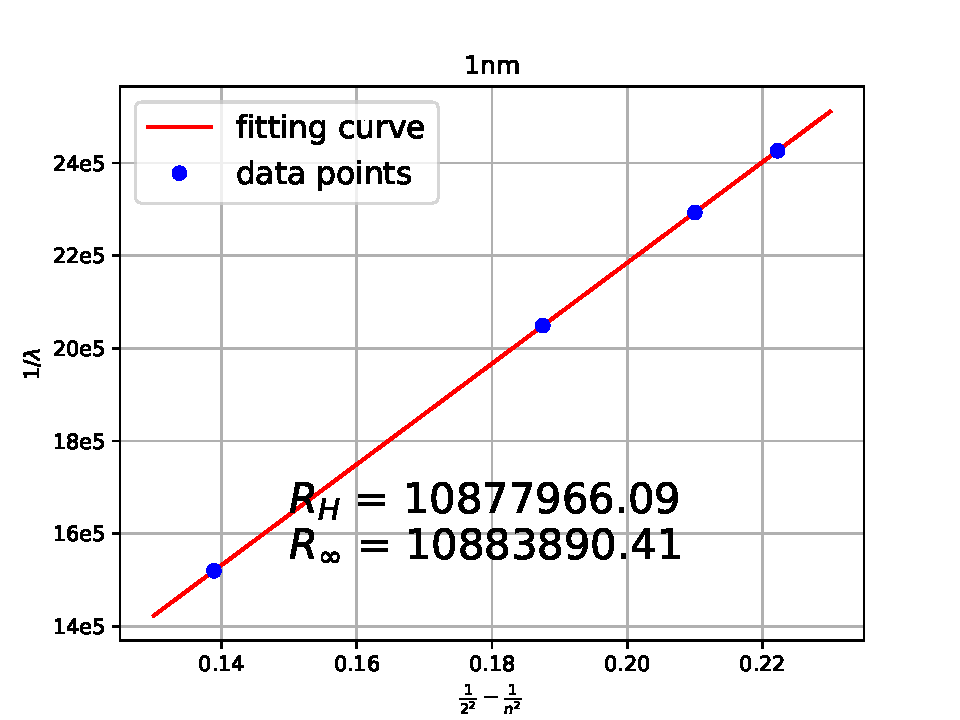
\includegraphics[width=10cm]{fig/fitting1nm.pdf}\\
\caption{1nm拟合曲线}\label{fitting1}
\end{figure}
\begin{figure}[!h]
\centering
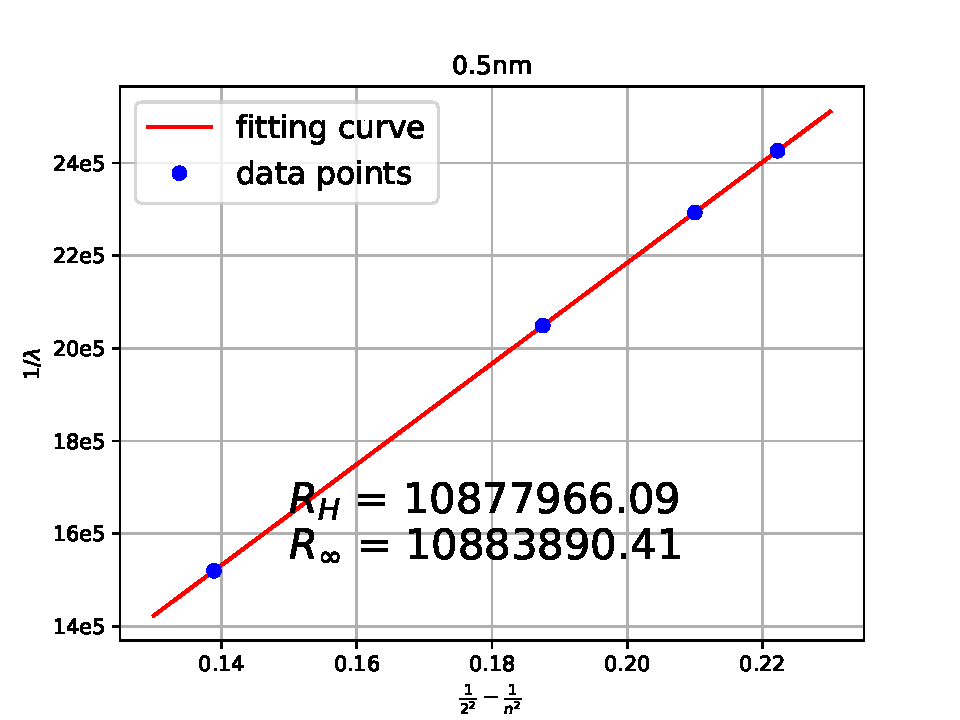
\includegraphics[width=10cm]{fig/fitting05nm.pdf}\\
\caption{0.5nm拟合曲线}\label{fitting05}
\end{figure}
\begin{figure}[!h]
\centering
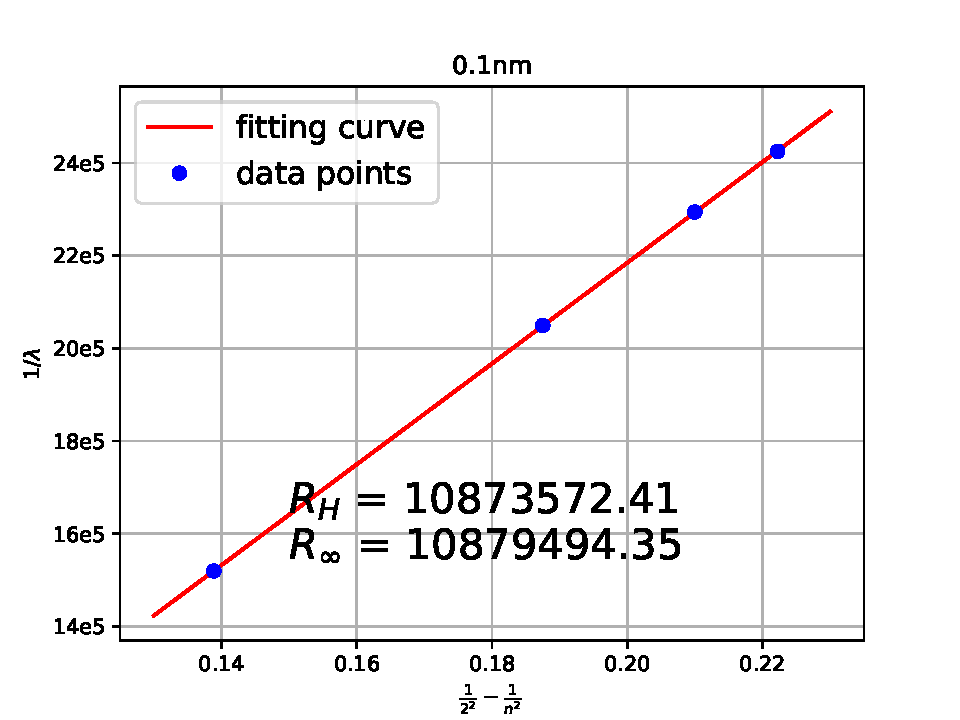
\includegraphics[width=10cm]{fig/fitting01nm.pdf}\\
\caption{0.1nm拟合曲线}\label{fitting01}
\end{figure}

其误差分别为:
\begin{eqnarray}
Error(1nm) &=& \cfrac{10883890.41 - 10973731.57}{10973731.57}\times 100\% \approx -0.819\%\\
Error(0.5nm) &=& \cfrac{10883890.41 - 10973731.57}{10973731.57}\times 100\% \approx -0.819\%\\
Error(0.1nm) &=& \cfrac{10879494.35 - 10973731.57}{10973731.57}\times 100\% \approx -0.859\%
\end{eqnarray}
可见拟合的误差是比较大的,我们再用测量数据直接进行计算,可得:

\begin{enumerate}
\item 1nm\\
$R_{\infty\alpha}$ = 10940320.55$\text{m}^{-1}$\\
$R_{\infty\beta} = $10926252.57$\text{m}^{-1}$\\
$R_{\infty\gamma}$ = 10918394.17$\text{m}^{-1}$\\
$R_{\infty\delta}$ = 10917533.80$\text{m}^{-1}$,\\
$<R_{\infty}>$ = 10925625.27$\text{m}^{-1}$\\
Error(1nm) = $\cfrac{10925625.27 - 10973731.57}{10973731.57}\times 100\% \approx -0.44\%$
\item 0.5nm\\
$R_{\infty\alpha}$ = 10940320.55$\text{m}^{-1}$\\
$R_{\infty\beta} = $10926252.57$\text{m}^{-1}$\\
$R_{\infty\gamma}$ = 10918394.17$\text{m}^{-1}$\\
$R_{\infty\delta}$ = 10917533.80$\text{m}^{-1}$,\\
$<R_{\infty}>$ = 10925625.27$\text{m}^{-1}$\\
Error(0.5nm) = $\cfrac{10925625.27 - 10973731.57}{10973731.57}\times 100\% \approx -0.44\%$
\item 0.1nm\\
$R_{\infty\alpha}$ = 10940320.55$\text{m}^{-1}$\\
$R_{\infty\beta} = $10928491.46$\text{m}^{-1}$\\
$R_{\infty\gamma}$ = 10923403.35$\text{m}^{-1}$\\
$R_{\infty\delta}$ = 10912238.92$\text{m}^{-1}$,\\
$<R_{\infty}>$ = 10926113.57$\text{m}^{-1}$\\
Error(0.1nm) = $\cfrac{10926113.57 - 10973731.57}{10973731.57}\times 100\% \approx -0.43\%$
\end{enumerate}
\end{enumerate}

\section{误差分析}
\iffalse
\begin{enumerate}
\item 实验室有自然光干扰。\\
在我们的实验过程中,观察到第一次实验时测量的谱线强度曲线通常不能观察到陡峭的峰值,而是一段较连续的平台,我们经研究推测是室内的环境光造成的影响。因为实验所测的氢原子光谱巴耳末线系的前四条谱线的波长均在可见光范围内,因此环境中的可见光可能对实验探测造成影响。为此,我们将探测器四周做好遮光,再次测量获得了非常理想的谱线强度曲线。
\item 仪器调节中狭缝光路调节存在误差。\\
第一次实验中我们还发现发光的氢灯管并没有对准探测器的接收窗口,因此也对测量造成了影响。后将氢灯管仔细调节,使接收窗口较为准确地与氢光灯相对,测量数据较好。但是因此我们也认为此装置在调节过程中还有可能存在调节不准的地方,造成误差。
\end{enumerate}
\fi

\section{思考题}
\subsection{氢光谱巴尔末线系的极限波长是多少?}
\subsection{谱线计算值具有唯一的波长,但实测谱线有一定宽度,其主要原因是什么? }

\nocite{jiaocai}
\bibliography{ref}
\end{document}